\documentclass[11pt,aspectratio=43,ignorenonframetext,t]{beamer}

% Presentation settings
\mode<presentation>{
  \usetheme[framenumber,titleframestart=1]{UoM_alex}
  \usefonttheme{professionalfonts} % using non standard fonts for beamer
  \usefonttheme{serif}             % set font to Arial
  \usepackage{fontspec}
  \setmainfont[Ligatures=TeX]{Arial}
}

% Handout settings
\mode<article>{
  \usepackage{fullpage}                  % use full page
  \usepackage{fontspec}                  % set font to Arial
    \setmainfont[Ligatures=TeX]{Arial}
  \setlength{\parskip}{1.5\baselineskip} % correct beamer line spacings
  \setlength{\parindent}{0cm}
  \usepackage{enumitem}
    \setlist[itemize]{topsep=0pt}
  \definecolor{uomlinkblue}{HTML}{0071BC}
}


% Packages

% Configurando layout para mostrar codigos C++
\usepackage{listings}
\lstset{
  language=Java,
  basicstyle=\fontsize{8}{10}\ttfamily, 
  keywordstyle=\color{blue}, 
  stringstyle=\color{orange}, 
  commentstyle=\color{gray}, 
  extendedchars=true, 
  showspaces=false, 
  showstringspaces=false, 
  numbers=left,
  numberstyle=\tiny,
  breaklines=true, 
  backgroundcolor=\color{blue!7},
  breakautoindent=true, 
  captionpos=b,
  xleftmargin=0pt,
}

\usepackage{graphicx}  % for graphics files
\usepackage{amsmath}   % assumes amsmath package installed
  \allowdisplaybreaks[1] % allow eqnarrays to break across pages
\usepackage{amssymb}   % assumes amsmath package installed 
\usepackage{hyperref} % add hyperlinks to document. Settings are for accessiblity
  \hypersetup{
    colorlinks=true,
    linkcolor=uomlinkblue,
    filecolor=uomlinkblue,      
    urlcolor=uomlinkblue,
	pdflang={en-GB},
}
\usepackage[document]{ragged2e} % left aligned text for accessibility
% experimental - does fundamentally work, if with quite a bit of effort
%\usepackage{axessibility} % LaTeX readable equations for accessibility
%  \tagpdfsetup{tabsorder=structure,uncompress,activate-all,interwordspace=true}
%  \pdfextension catalog{/Lang (en-GB)}
%  \RequirePackage{luacode}
%  \directlua{require("axessibility.lua")}
\usepackage{unicode-math} % unicode maths for accessibility
\usepackage{pdfcomment} % for alt text for accessibility
\usepackage{rotating}  % allow portrait figures and tables
\usepackage{subfigure} % allow matrices of figures
\usepackage{float}     % allows H option on floats to force here placement
\usepackage{multirow}  % allows merging of rows in tables
\usepackage{tabularx}  % allows fixed width tables
\usepackage{ctable}    % modifies \hline for use in table
\usepackage{bm}        % allow bold fonts in equations
\usepackage{pgf}       % allow graphics manipulation
\usepackage{media9}    % allow interactive flash files to be embedded
  \addmediapath{../media}
\usepackage{etoolbox}
  \makeatletter \preto{\@verbatim}{\topsep=0pt \partopsep=0pt} \makeatother  
  
% Custom commands
\newcommand{\matlab}{\emph{\sc{Matlab}}}
\newcommand{\maple}{\emph{\sc{Maple}}}
\newcommand{\simulink}{\emph{\sc{Simulink}}}
\newcommand{\dc}{d.c.}
\newcommand{\ac}{a.c.}
\newcommand{\rms}{RMS}
\newcommand{\wgn}{{\tt wgn}}
\newcommand{\sus}[1]{$^{\mbox{\scriptsize #1}}$}
\newcommand{\sub}[1]{$_{\mbox{\scriptsize #1}}$}
\newcommand{\chap}[1]{Chapter~\ref{#1}}
\newcommand{\sect}[1]{Section~\ref{#1}}
\newcommand{\fig}[1]{Fig.~\ref{#1}}
\newcommand{\tab}[1]{Table~\ref{#1}}
\newcommand{\equ}[1]{(\ref{#1})}
\newcommand{\appx}[1]{Appendix~\ref{#1}}
\newcommand{\degree}{\ensuremath{^\circ}}
\newcommand{\Vrms}{Vrms}
\newcommand{\Vpp}{V\sub{pp}}
\newcommand{\otoprule}{\midrule[\heavyrulewidth]}         
\newcolumntype{Z}{>{\centering\arraybackslash}X}  % tabularx centered columns 
\makeatletter \DeclareRobustCommand{\em}{\@nomath\em \if b\expandafter\@car\f@series\@nil \normalfont \else \bfseries \fi} \makeatother
\newcounter{example_number} % keep track of the example questions



%%%%%%%%%%%%%%%%%% FRONT MATTER %%%%%%%%%%%%%%%%%%
\title{Desenvolvimento de Software}
\subtitle{Aula 20 - Tratamento de Exceções}
\author{Prof. Me. Juliana Costa-Silva}

\begin{document}

\maketitle
%%%%%%%%%%%%%%%%%% TITLE SLIDE %%%%%%%%%%%%%%%%%%
\mode<presentation>{ \frame{\titlepage \label{slide:a}}} 
%\begin{figure}[!ht] 
%\fbox{\includeslide[width=\textwidth]{slide:a}} \end{figure}

%------------------------------------------------------------------------
\mode<presentation>{
\begin{frame}
\frametitle{Na aula de hoje...} 
\tableofcontents 
\end{frame}
}

\section{Introdução}
\begin{frame}{Na última aula...}
 \begin{itemize}
  \item Interfaces 
  \item Revisão de interfaces
  \item Atividades 
 \end{itemize}
\end{frame}
%------------------------------------------------------
\begin{frame}{Exceção}{Conceito}
  \begin{block}{o que é?}
      Indicação de um problema que ocorre durante a execução de um programa \cite{deitel2017java}.
  \end{block}

\end{frame}
%-------------------------------------------------------------
\begin{frame}{O que pode gerar uma exceção?}
    \begin{block}{Usuário}
        \begin{itemize}
            \item Divisão por zero;
            \item Caracteres inválidos;
        \end{itemize}
    \end{block}
    \begin{block}{Código}
        \begin{itemize}
            \item Senha de acesso ao banco de dados errada;
            \item Tentativa de abrir um arquivo inexistente;
            \item Manipulação de variável com valor null (sem objeto);
        \end{itemize}
    \end{block} 
\end{frame}
%-----------------------------------------------------------
\section{Tratamento de Exceções - Conceito}
\begin{frame}{Tratamento de Exceções}{Conceito}
    Mecanismo utilizado para identificar e tratar possíveis  exceções;
    \begin{itemize}
        \item Permite que o programa continue executando;
        \item Possibilita o desenvolvimento de aplicações tolerante a falhas;
    \end{itemize}
\end{frame}

%-----------------------------------------------------------
\begin{frame}{Tratamento de Exceções}{Conceito}
    As exceções em Java são \textbf{objetos}! Todas as classes de exceção Java herdam direta ou indiretamente da classe \textbf{Expception}.
   \begin{center}
  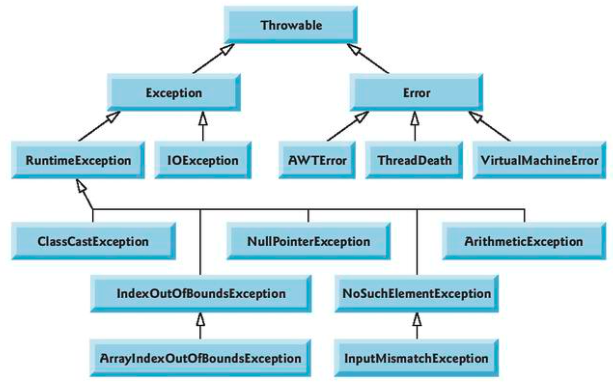
\includegraphics[height=0.5\paperheight]{fig/aula20/aula20_1.png} \\
 \end{center}
\end{frame}
%-----------------------------------------------------------
\section{Tratamento de Exceções - Aplicações}
\begin{frame}{Tratamento de Exceções}{Aplicações}
\begin{itemize}
    \item Somente objetos \textbf{Throwable} podem ser utilizados como mecanismo de tratamento de exceção. 
    \item A classe \textbf{Throwable} tem duas subclasses diretas: \textbf{Exception} e \textbf{Error}. 
    \item A classe \textbf{Exception} e suas subclasses -exemplo, RuntimeException (pacote java.lang ) e IOException (pacote java.io) - representam situações excepcionais que podem ocorrer em um programa Java e que podem ser capturadas pelo aplicativo. 
\end{itemize}
\tiny{Fonte: \cite{deitel2017java}}.
\end{frame}
%-----------------------------------------------------------
\begin{frame}{Tratamento de Exceções}{Aplicações [2]}
\begin{itemize} 
    \item A classe \textbf{Error} e suas subclasses representam situações anormais que acontecem na JVM. 
    \item A maioria dos \underline{Errors} acontece com pouca frequência e não deve ser capturada pelos aplicativos — geralmente os aplicativos não podem se recuperar de \underline{Errors}.
\end{itemize}
\tiny{Fonte: \cite{deitel2017java}}.
\end{frame}
%----------------------------------------------------------
\begin{frame}{Métodos de exceções}
\textbf{Throwable} é classe base de todas as exceções. \\
Esta classe fornece os métodos:
\begin{itemize}
    \item getMessage() – retorna mensagem do erro;
    \item printStackTrace() – retorna a pilha de métodos chamados;
    \item toString() - retorna uma string com a descrição da exceção;
\end{itemize}
\end{frame}
%------------------------------------------------------
\section{Prática}
\begin{frame}{Tratando exceções}
    \begin{center}
        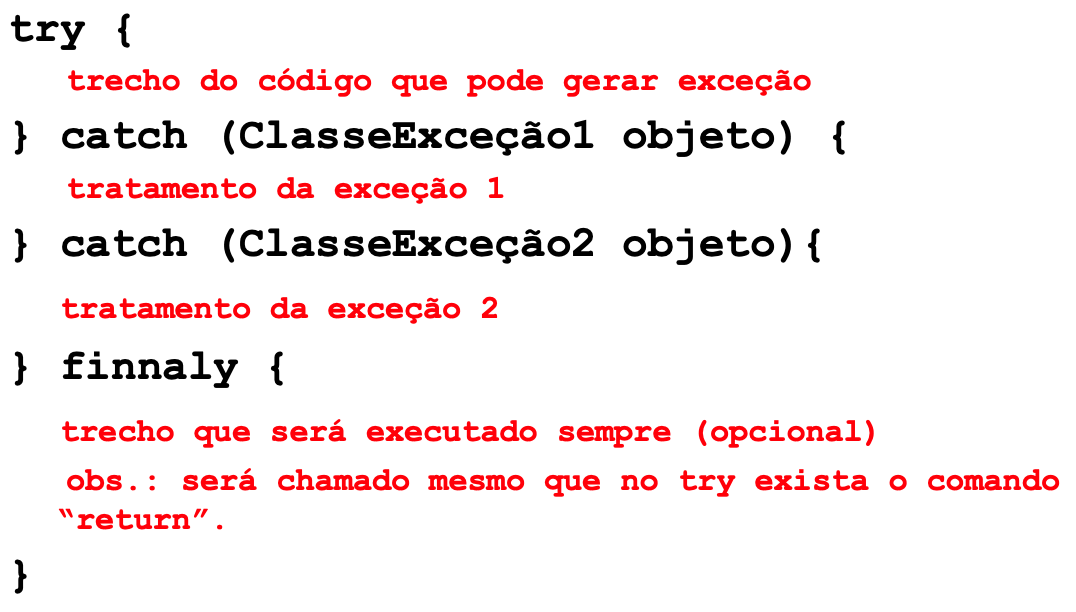
\includegraphics[height=0.7\paperheight]{fig/aula20/try_catch.png} \\
    \end{center}  
\end{frame}
%----------------------------------------------
\begin{frame}{Métodos tratando exceções}
    Métodos podem definir exceções que podem gerar (disparar):
    \begin{itemize}
        \item O comando throw “dispara” a exceção;
        \item O comando throws é colocado no método, seguido dos tipos de exceções que pode disparar;
        \item O trecho do código que chamou o método deve tratar a exceção
    \end{itemize}
\end{frame}
%-----------------------------------------------------------
\section{Leitura recomendada}
\begin{frame}{Leitura complementar}
 Para mais informações sobre abstract e final em JAVA, leia:\\
 \begin{columns}
   \begin{column}{0.4\textwidth}
     Java: Como programar\\
     Capítulo 10: \cite{deitel2010java}\\
     \vspace{0.3cm}
      Java para Iniciantes\\
      Capítulo 6
      \cite{schildt2015java}
   \end{column}
   \begin{column}{0.3\textwidth}
    \begin{center}
  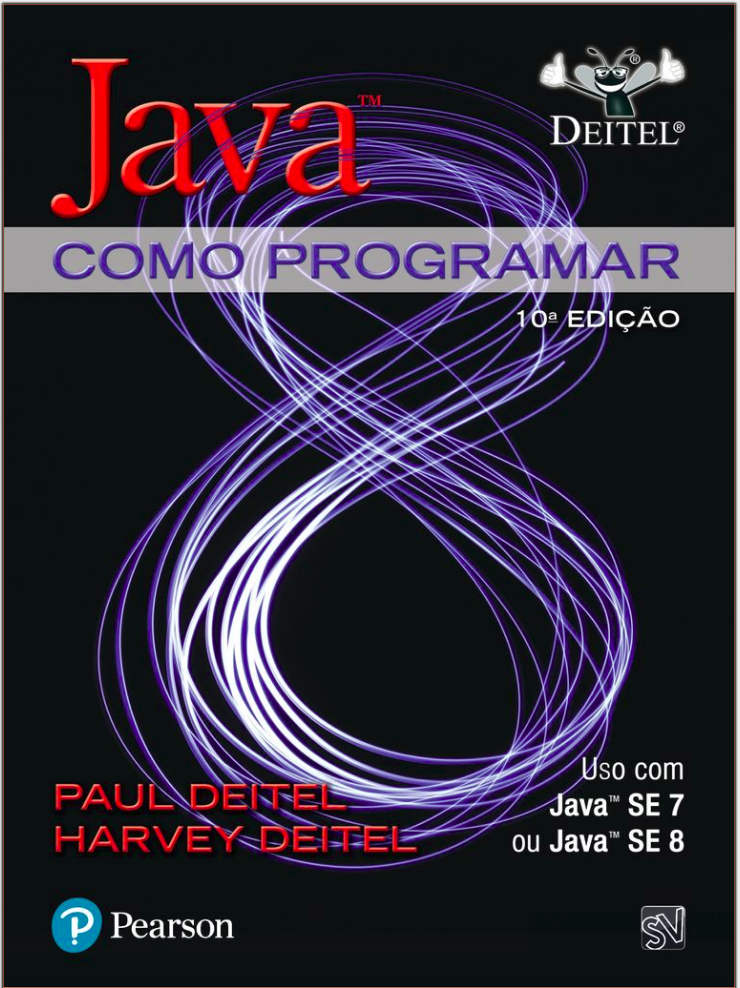
\includegraphics[height=0.5\paperheight]{fig/aula1/deitel2017java.png} \\
 \end{center}
   \end{column}
 \end{columns}
\end{frame}
%----------------------------------------------------------------------
\section{Referências}

\begin{frame}{Referências}%[allowframebreaks]
\small
\begin{center}
\tiny
\bibliographystyle{apalike}
\bibliography{ref_aula_progI}
\end{center}
\end{frame}
\setcounter{framenumber}{\thelastpagemainpart}

\end{document}